\section{UML Transformations}
\label{sec:umltransformations}

This section collects some transformations needed in a UML State-Machine
diagram (UML-SM) in order to fulfil the UML-SM subset defined in
Section~\ref{sec:umlsubset}. 

Recall that in the proposed UML-SM subset the only activities that can appear in
some state are {\tt do} activities. However, a UML-SM state, as defined
in~\cite{UML-OMG-11}, may have also {\tt entry} and {\tt exit} activities, that
are respectively executed upon entrance or exit of a state.

\begin{figure}
\centering
  \begin{tabular}{c}
  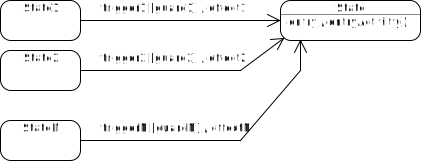
\includegraphics[width=0.7\columnwidth]{images/entryActionsBEFORE}\\ 
(a)\\
  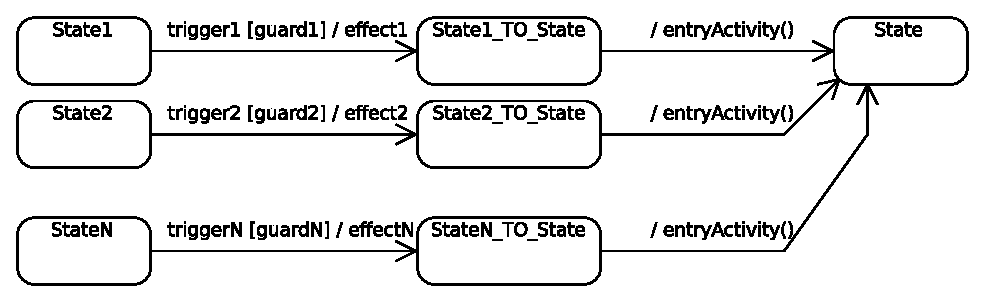
\includegraphics[width=0.85\columnwidth]{images/entryActionsAFTER}\\
(b)
  \end{tabular}
  \caption{Transformation performed for a {\em State} with an {\tt entry}
activity.}
  \label{fig:entryActions}
\end{figure}

Let us firstly consider a {\em State} having an {\tt entry} activity, as
shown in Figure~\ref{fig:entryActions}(a). Assume that there are $N$ states
({\em State1}, {\em State2}, \ldots, {\em StateN}) that lead to {\em State} when
some guard is fulfilled and triggered, having also associated some effect. The
transformation is performed as follow: for each incoming transition to {\em
State}, a new state is added. This new state is the destination of the incoming
transition, leaving the transition signature (i.e., its trigger, guard and
effect information) as in the original model. Finally, an output transition is
added to the new state that leads to {\em State}. This output transition has no
guard nor trigger event but an effect that correspond to the {\tt entry}
activity of {\em State} before the transformation.
Figure~\ref{fig:entryActions}(b) depicts the transformation performed in a
 model where a {\em State} has an {\tt entry} activity
(Figure~\ref{fig:entryActions}(a)).


\begin{figure}
\centering
  \begin{tabular}{c}
  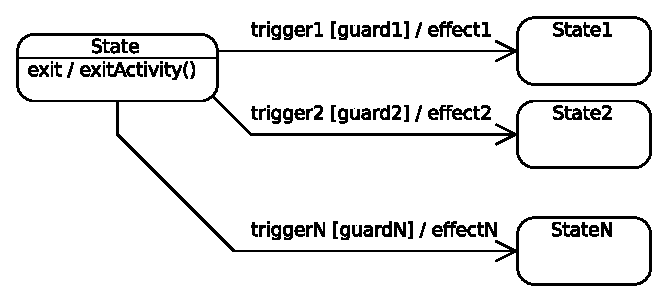
\includegraphics[width=0.7\columnwidth]{images/exitActionsBEFORE}\\ 
(a)\\
  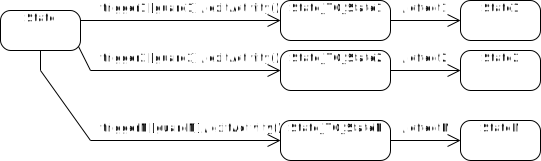
\includegraphics[width=0.85\columnwidth]{images/exitActionsAFTER}\\
(b)
  \end{tabular}
  \caption{Transformation performed for a {\em State} with an {\tt exit}
activity.}
  \label{fig:exitActions}
\end{figure}

Let us consider now a {\em State} having an {\tt exit} activity, as
shown in Figure~\ref{fig:exitActions}(a). Assume that a {\em State} with an
{\tt exit} activity has $N$ different output transitions, each one leading to
different states and being triggered by different event, having a guard and an
effect activity in the transition. In this case, the transformation is
performed as follows: for each output transition of {\em State}, a new states
is added. This new state is the destination of the output transition having as
signature the trigger and the guard of the original model, but changing the
effect to the {\tt exit} activity. Finally, an output transition is added to
the new state leading to the outputs state of the original model. This output
transition has no guard nor trigger event but an effect that correspond to the
effect that was performed when transiting to each state from {\em State} in the
original model. Figure~\ref{fig:exitActions}(b) depicts the transformation
performed in a  model where a {\em State} has an {\tt exit} activity
(Figure~\ref{fig:exitActions}(a)).


\begin{figure}
  \centering
  \begin{tabular}{c}
  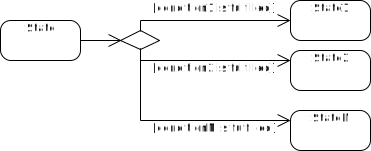
\includegraphics[width=0.7\columnwidth]{images/choiceBEFORE}\\ 
(a)\\
  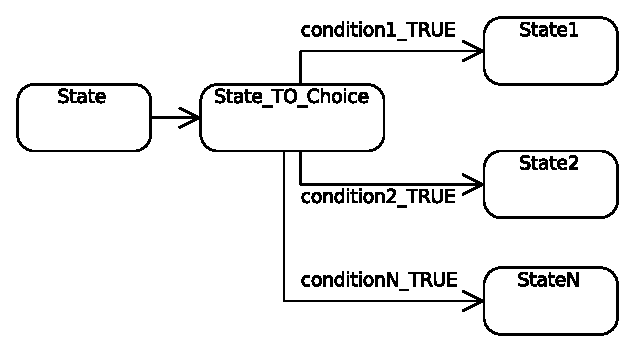
\includegraphics[width=0.7\columnwidth]{images/choiceAFTER}\\
(b)
  \end{tabular}
  \caption{Transformation performed for a {\em State} with a {\tt choice} 
pseudo-state.}
  \label{fig:choicePseudostate}
\end{figure}

Another UML-SM element that we consider in this paper is the {\tt choice}
pseudo-state. A {\tt choice} pseudo-state realises a dynamic conditional
branch, evaluating the guards of the triggers of its outgoing transitions to
select only one outgoing transition. In the case of having more than one
outgoing transitions, any of them can be selected.

Figure~\ref{fig:choicePseudostate}(a) shows a {\em State} having an output {\tt
choice} pseudo-state. Assume that $N$ conditions, when fulfilled, are leading to
a new state. In this case, the transformation is
performed as follows: the {\em choice} pseudo-state is transformed to a state,
having \TODO{\ldots}

